\chapter{The Discrete Fourier Transform and Fast Fourier Transform}
Frequency domain analysis is widely used in the DSP area, a signal in time domain is transformed to frequency domain by means of the DFT. Since the direct implementation of the DFT is time consuming and due to the widely range of applications of the DFT, several algorithms called of Fast Fourier Transforms originated. Fast Fourier algorithms decrease the DFT complexity (fewer operations and/or simpler computations tasks) by means of a divide and conquer approach. Essentially it maps the problem into several sub-problems and applies the division recursively to the sub-problems as well, eventually leading to a reduction in computation complexity. 

Fast algorithms can be classified in two major classes, those based on the Good's mapping, which basically factors the DFT or divides the DFT into smaller DFTs with its sizes being co-prime, this approach has the advantage of no producing any Twiddle Factor (equation \ref{eq:twiddle}), with this a lower bound in complex multiplications is achieved, the Winograd Fourier Transform (\ac{wfta})~\cite{winograd1978computing} and Prime Factor algorithm (\ac{pfa})~\cite{pfa_fft} are two of the algorithms based on this method. A second class of algorithms known as Cooley-Tukey Fast Fourier Transform (\ac{ctfft}) or radix-r algorithms, suitable for $r^n$ size sequences, where the use of twiddle factors is inevitable.

CTFFT algorithms adds regularity to the computation, considering that CTFFT algorithms show a more repetitive use of fewer modules, and are easier to implement in a parallel kind of way, since the small repetitive modules are applied on contiguous sets of data. This also is advantageous since improvements in those small repetitive blocks allows from an overall improvements of the computation. Moreover, CTFFT algorithms are more suitable for in-place computation, a desired feature since no additional memory is required. On the other hand, algorithms like the WTFA requires huge memory and does not allow for in-place computation~\cite{duhamel1990fast}. 


All the advantages of the CTFFT algorithms over Good's based ones, lead to Cooley-Tukey algorithms begin more used in implementations. Complex multiplications alone are not the main concern in implementation and computation time, number of additions, memory access, communications costs are examples of other variables that are at least as important. It is worth noticing that while a lot of research have been done in the subject due to the importance of the DFT and FFT algorithms, new algorithms continue to emerge as is the case of the Sparse Fourier Transform presented in \cite{sfft_paper} and implemented in \cite{milion_point_sfft} for a million point DFT. This algorithms takes advantage of the sparsity shown in some signal where the DFT is applied, that is, only a phew components of the signal are of importance since all other signal components in frequency domain are zero, the algorithm then only computes the set of needed non-zero frequency components. This is not the case of the current intended application, therefore, the classic approach to the FFT implementation is adopted. In the following, a review of the Cooley-Tukey approach to the DFT computation is presented.




\section{FFT Cooley-Tukey Algorithm}




The DFT is a mathematical tool widely used in signal processing. Basically, the DFT of a \textit{N}-point sequence converts discrete samples from time-domain to frequency-domain and vice versa through equation \ref{eq:dft}: 

 \begin{equation} 
     X[k]=\sum _{n=0}^{N-1} x[n]W^{nk}_N,
     \label{eq:dft}
 \end{equation}
where $k =0,1,2,\cdots,\textit{N}-1$ and $W_N$ (also known as twiddle factor)
is given by:
 \begin{equation} 
     W_N= \textit{e}^{\frac{-j2\pi}{N}}.
     \label{eq:twiddle}
 \end{equation}
An \textit{N}-point inverse DFT (IDFT) is computed as: 
 \begin{equation} 
     x[n]=\frac{1}{N}\sum _{k=0}^{N-1} X[k]W^{-nk}_N.
     \label{eq:idft}
 \end{equation}

The direct computation of the DFT is difficult to implement due to its high computation complexity, for instance, a $N$ points computation of a sequence composed of complex samples requires $N^2$ complex multiplications (each complex multiplication is equal to $4$ real multiplications and $2$ real additions) and $N^2-N$ complex additions (every complex addition is equal to $2$ real additions), a complexity of $O(N^2)$~\cite{proakis1996digital}. 

% Based on the symmetry(eq \ref{eq:twidle_sym}) and periodicity  (eq \ref{eq:twidle_period}) property of the twiddle factor and a divide-and-conquer approach a new class of algorithms that optimizes the computation of the DFT were developed \cite{cooley_fft}, this new class of algorithms are known as Fast Fourier Transform (FFT). The Cooley and Turkey algorithm is a well known FFT algorithm, in the next section a description of the algorithm is presented.


%  \begin{equation} 
%      \centerline{Symmetry: ${W}_{N}^{k+N/2} = -{W}_{N}^{k}$}
%      \label{eq:twidle_sym}
%  \end{equation}


% \begin{equation} 
% \centerline{Periodicity: ${W}_{N}^{k+N} = {W}_{N}^{k}$}
% \label{eq:twidle_period}
% \end{equation}

Based on a divide-and-conquer approach a new class of algorithms that optimizes the computation of the DFT were developed, this new class of algorithms are known as Fast Fourier Transform (FFT). The Cooley and Turkey\cite{cooley_1965} algorithm is a well known FFT algorithm.

The divide and conquer approach divides the computation problem in smaller problems, and solves every smaller problem recursively using the same algorithm, the solution to the original problem is then the combination of the smaller solutions. A common approach is to divide the problem by half, then each half is then divided by half, and so on. This is known as radix-2 FFT, the partition goes until only size two DFTs remain. Following this approach two type of FFTs are derived according to the domain where the division is performed, the Decimation in Time (DIT), where the partition occurs on the input sequence (time domain), and the Decimation in Frequency (DIF) where the output sequence is partitioned (frequency domain). 

%Two kinds of FFT algorithms are found in the literature, a decimation in time FFT, which divides the input sequence into even and odds samples iteratively until only size $2$ DFTs are computed, and the decimation in frequency which uses a similar approach, only that in this case the decimation is performed over the frequency samples. When the decimation is performed in pairs it is called Radix-2, higher radixes FFTs are also used, where only size $r$ ($r$ beign an integer multiple of $2$) DFTs are computed after the decimation process, either in time or frequency domain.       

The decimation in frequency algorithm is derived as follows,  given a $x(n)$ sequence of length $N = 2^p$, where $p$ is an integer, the DFT of a time sequence $x(n)$ computed as in eq.~\ref{eq:dft} can be written as:

\begin{equation} 
\begin{split}
     X[k]=\sum _{n=0}^{N/2-1} x[n]W^{nk}_N + \sum _{n=N/2}^{N} x[n]W^{nk}_N  \\  =\sum _{n=0}^{N/2-1} x[n]W^{nk}_N + W^{Nk/2}_N\sum _{n=0}^{N/2-1} x[n+N/2]W^{nk}_N,
     \label{eq:dft2}
     \end{split}
\end{equation}

% \begin{multline} 
%      X[k]=\sum _{n=0}^{N/2-1} x[n]W^{nk}_N + \sum _{n=N/2}^{N} x[n]W^{nk}_N  \\  =\sum _{n=0}^{N/2-1} x[n]W^{nk}_N + W^{nk/2}_N\sum _{n=0}^{N/2-1} x[n+N/2]W^{nk}_N,
% \end{multline}
 Since ${W}_{N}^{Nk/2} = (-1)^k$ eq.~\ref{eq:dft2} can be written as:

\begin{equation} 
     X[k]=\sum _{n=0}^{N/2-1} [x(n) + (-1^{k})x(n+N/2)]W^{nk}_{N}
\label{eq:dft_even}
\end{equation}

Decimating in frequency (i.e. splitting in odds and even frequency components) and using the fact that ${W}_{N}^{2} = {W}_{N/2}^{}$, 


\begin{equation} 
     X[2k]=\sum _{n=0}^{N/2-1} [x(n) + x(n+N/2)]W^{nk}_{N/2}
\label{eq:dft_even}
\end{equation}


\begin{equation} 
     X[2k +1]=\sum _{n=0}^{N/2-1} [[x(n) - x(n+N/2)]W^{n}_{N}]W^{nk}_{N/2}
\label{eq:dft_odd}
\end{equation}


The entire coputation of the $N/2$ point sequences \ref{eq:dft_even} and \ref{eq:dft_odd} can be rewritten as: 

\begin{equation} 
     X[2k]=\sum _{n=0}^{N/2-1} g1(n)W^{nk}_{N/2}
\label{eq:dft_even2}
\end{equation}

\begin{equation} 
     X[2k+1]=\sum _{n=0}^{N/2-1} g2(n)W^{nk}_{N/2}
\label{eq:dft_odd2}
\end{equation}

where 

\begin{equation} 
  g1(n) = [x(n) + x(N/2 + n)]
\label{eq:dft_btfly1}
\end{equation}

\begin{equation} 
    g2(n) = [x(n) - x(N/2 + n)]W^{nk}_{N/2}
\label{eq:dft_btfly2}
\end{equation}

Fig.~\ref{fig:dif_1}, shows an example of the computation of eq.~\ref{eq:dft_odd} and \ref{eq:dft_even} for a 8 point sequence. It can be seen as two DFTs of half the sequence size, with two input sequences given by eq.~\ref{eq:dft_btfly1} and eq.~\ref{eq:dft_btfly2}.

\begin{figure}[htbp]
  \centering
   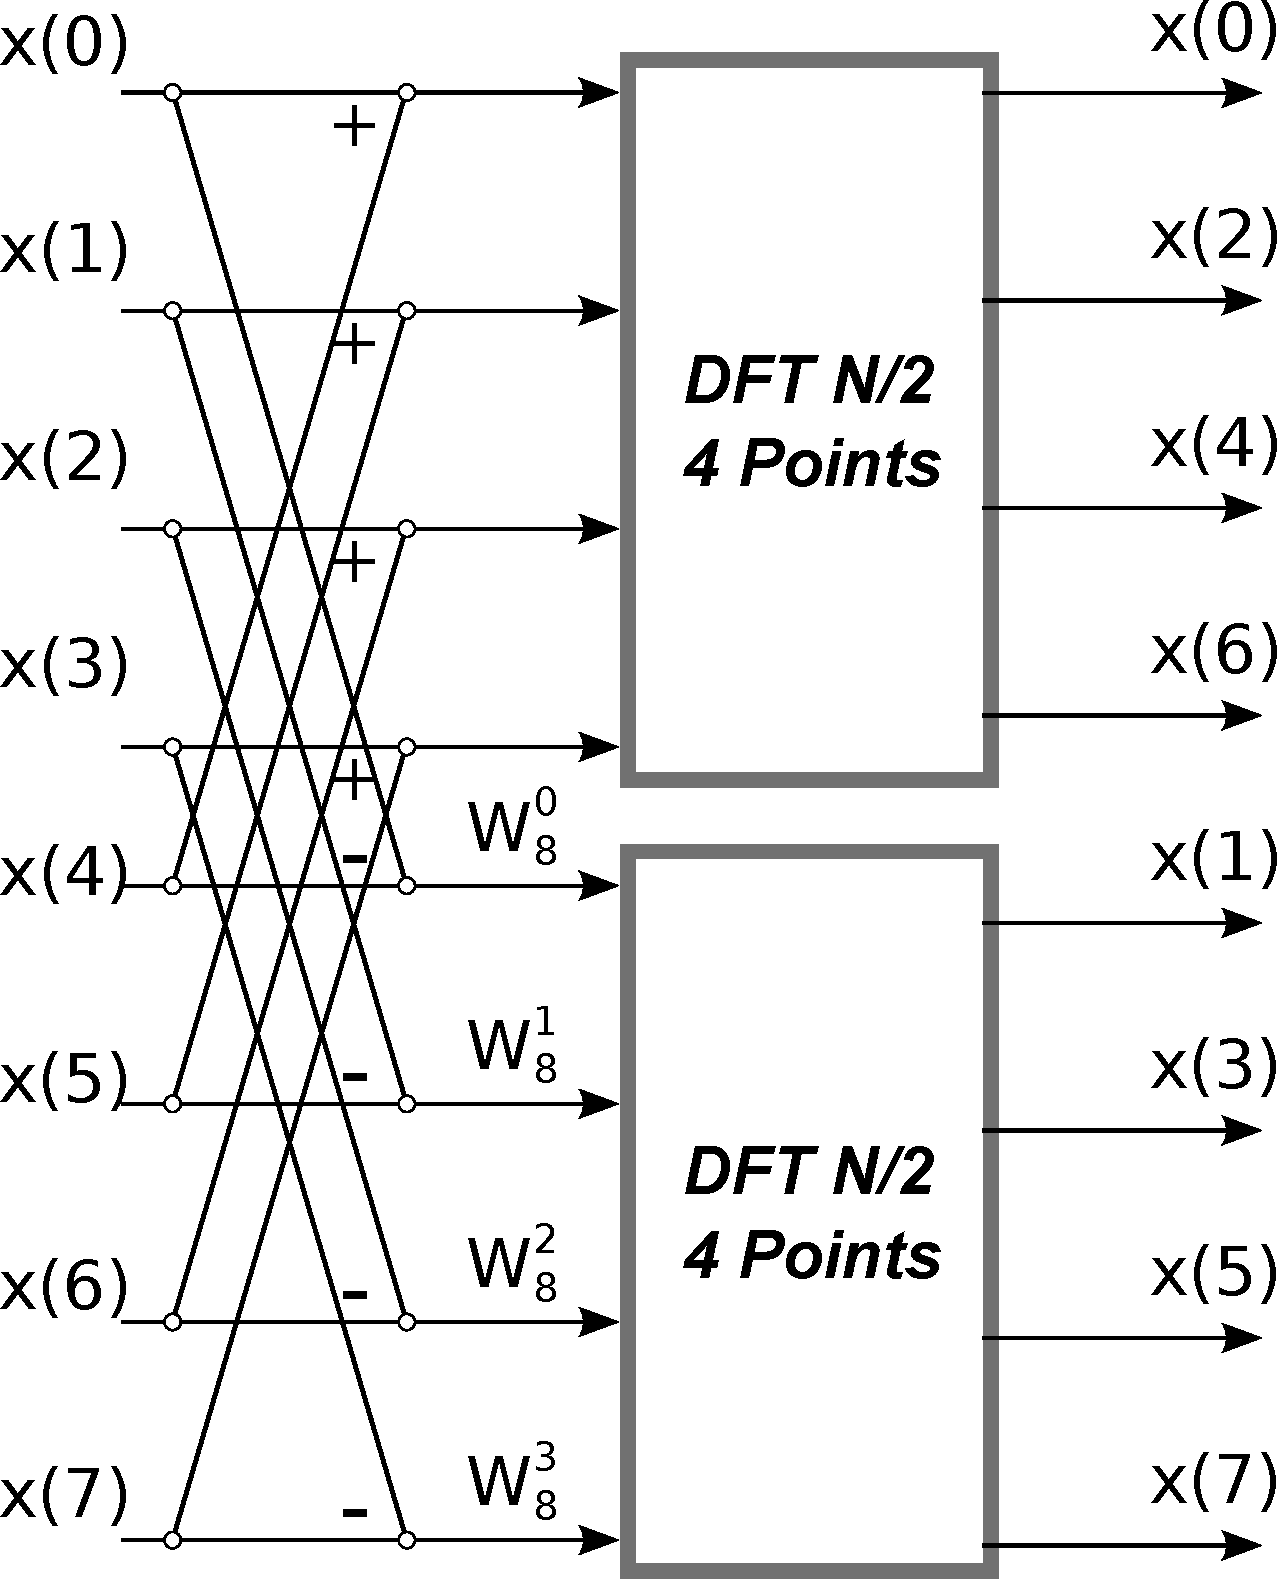
\includegraphics[width=0.4\textwidth]{./figures/fft_partial_dif}
    %\rule{35em}{0.5pt}
  \caption{First stage in the DIF computation process}
  \label{fig:dif_1}
\end{figure}

Performing the same computations on the $N/2$ point DFTs until only remains two points DFTs, an optimization in the algorithm can be made. Fig.~\ref{fig:dif_diagram} shows a diagram of the entire computation process for a DFT of size 8 using the FFT. It can be seen highlighted the basic computation process performed in every stage, two complex samples are added, subtracted and multiplied by the twiddle factor. This operation is known as the butterfly (fig. \ref{fig:DIF_btfly}), and it involves one complex multiplication and two complex additions.    

\begin{figure}[htbp]
  \centering
   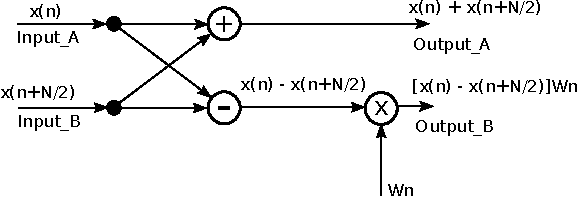
\includegraphics[width=0.6\textwidth]{./figures/btfly}
    %\rule{35em}{0.5pt}
  \caption{Decimation in frequency butterfly}
  \label{fig:DIF_btfly}
\end{figure}

There are $N/2$ butterflies per stage and $log2(N)$ stages. Thus,  the total number of complex multiplications is $N/2log2(N)$ and complex additions is $Nlog(N)$ which is much less than $N^2$ complex multiplications and $N^2-N$ complex additions of the direct implementation, this algorithm shows a complexity of $O(N/2log2(N))$. The optimization of the algorithms relies on the redundancy present on the twiddle factor which is exploited consequently using less multiplications to perform the computation. Higher radices (4, 8, 16) can be derived when the division of the sequence done by $2^n$ $n = 1, 2, 3, 4, .. etc$. Fewer multiplications at the cost of a more complex butterfly and control of the entire computations is achieved with higher radices.  In the next section the implications of the hardware implementation of the FFT algorithm is addressed. 

\begin{figure}[htbp]
  \centering
   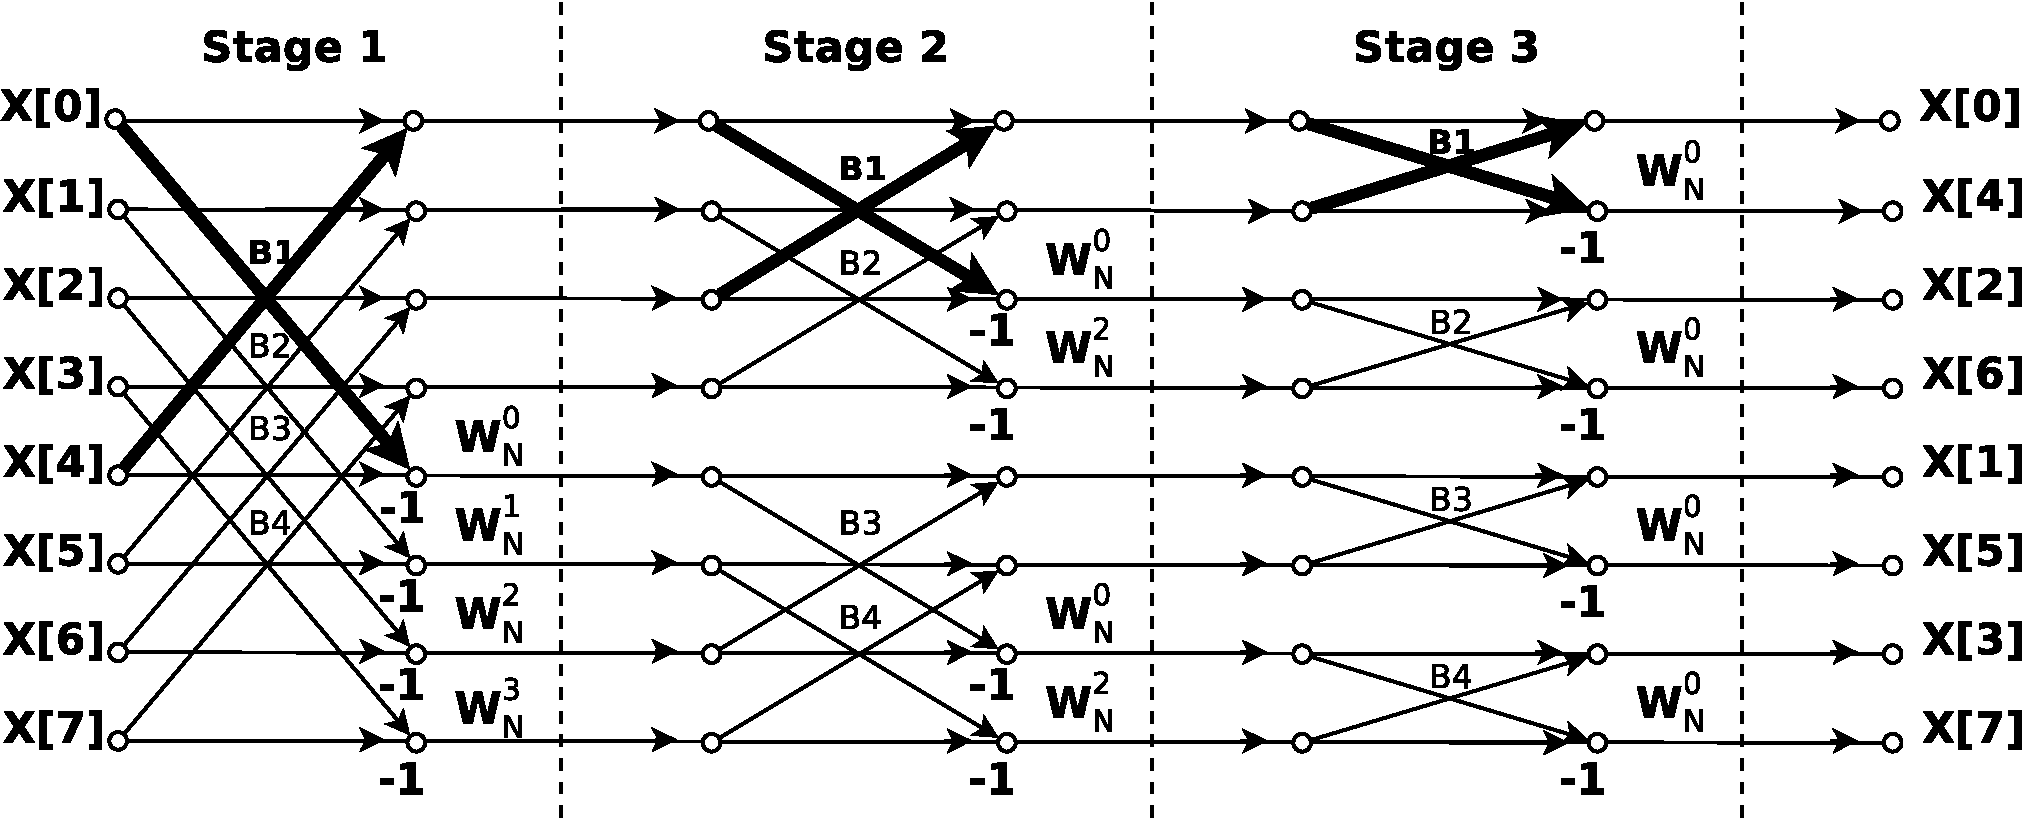
\includegraphics[width=1\textwidth]{./figures/DIF_FFT.pdf}
    %\rule{35em}{0.5pt}
  \caption{Decimation in frequency diagram}
  \label{fig:dif_diagram}
\end{figure}

